\documentclass[11pt]{article}

\usepackage[margin=1in]{geometry}
\usepackage{amsmath,amssymb}
\usepackage{graphicx}
\usepackage{booktabs}
\usepackage{authblk}
\usepackage{microtype}
\usepackage[style=authoryear,backend=biber,natbib=true,maxcitenames=2,uniquename=false]{biblatex}
\usepackage[colorlinks=true,allcolors=blue]{hyperref}

\graphicspath{{figures/}}
\addbibresource{references.bib}

\newcommand{\Rdep}{R_{\mathrm{dep},t}}
\newcommand{\Rg}{R^{\mathrm{guide}}_t}
\newcommand{\Rd}{R^{\mathrm{donor}}_t}
\newcommand{\Rc}{R^{\mathrm{condition}}_t}

\title{\textbf{Reliability-weighted target prioritization in CD4+ T-cell
Perturb-seq: a generalizability-theory decomposition}}

\author[1]{Che Cheng}
\affil[1]{Institute of Statistical Science, Academia Sinica, Taipei, Taiwan.
\texttt{che830621@stat.sinica.edu.tw}. ORCID 0000-0003-3376-7833.}

\date{\today}

\begin{document}
\maketitle

\begin{abstract}
\noindent Genome-wide Perturb-seq screens prioritize candidate targets by the
strength of a perturbation's transcriptional effect. Effect strength does not
answer a prior measurement question: is the readout dependable? A large effect
estimated from a single guide, a single donor, or a pseudobulk of few cells need
not survive replication, and for target prioritization each false lead costs a
validation experiment. We treat each perturbation effect as a measurement in a
crossed Target $\times$ Guide $\times$ Donor $\times$ Condition design and apply
generalizability theory \parencite{cronbach1972} to separate the dependable part
of an effect from facet-specific idiosyncrasy. Guides and donors enter as random
facets; condition enters as a fixed facet and is analyzed within its levels. For
each target we report a dependability profile over the facets and a joint
generalizability coefficient over the two random facets, and we re-rank targets
by effect magnitude weighted by that coefficient. On the released screen
\parencite{zhu2025}, removing the measurement-error floor estimated from the
non-targeting controls raises the number of genes with a dependable target-signal
share above $.10$ from $40$ to $7{,}674$. A design study indicates that
reliability is limited by the number of guides rather than the number of donors.
Analyzed within activation states, dependability recovers the T-cell-receptor
signaling module as reliably measurable only in activated cells, without recourse
to gene annotation. Every methodological decision was recorded and adversarially
reviewed, and all results regenerate from the released summary statistics.
\end{abstract}

\section{Dependability, not effect size}

Target prioritization in Perturb-seq conventionally ranks candidates by
differential-expression strength: effect size, $z$-score, false-discovery rate,
or the number of downstream differentially expressed genes. These summaries
answer whether a perturbation moved the transcriptome \emph{in the observed
dataset}. They do not answer whether the effect would hold up under another
guide, another donor, or another cell-state context. The two questions come
apart. A target can carry a large apparent effect that is fragile, when two
guides disagree, one donor drives the signal, knockdown is weak, or an off-target
flag is present; a target of moderate effect that is consistent across guides and
donors can be the better validation bet. We therefore treat \emph{dependability}
as a first-class quantity alongside magnitude.

This concern is not new in high-throughput biology, though it has rarely been
framed as measurement reliability. \textcite{li2011idr} call discoveries by their
reproducibility across replicates rather than by effect size, defining an
irreproducible discovery rate as an analogue of the false-discovery rate;
\textcite{billmann2023} show that standard CRISPR-screen quality metrics do not
by themselves capture the reproducibility of context-specific hits; and
data-driven target-prioritization frameworks integrate several weighted evidence
types rather than fitness effect alone \parencite{behan2019}. Generalizability
theory supplies the missing piece: a single interpretable coefficient for the
dependability of a per-target effect, together with an explicit account of which
experimental facet limits it.

\section{A generalizability-theory decomposition}

\subsection{The crossed design and its facets}

The experimental structure maps onto a psychometric measurement design
\parencite{lordnovick1968}. The target gene is the object of measurement; the true
perturbation signature is the universe score; the two guides per gene act as
parallel forms; the four donors and the three culture conditions are crossed
facets; cell sampling and sequencing contribute residual error. Classical test
theory writes an observed score as $X = T + E$, its true score the expected
observation over independent replications \parencite{novick1966}; generalizability
theory \parencite{cronbach1972} decomposes the error term into named sources,
\[
E = E_{\mathrm{guide}} + E_{\mathrm{donor}} + E_{\mathrm{condition}}
      + E_{\mathrm{interactions}} + E_{\mathrm{residual}},
\]
and reports how much of the effect is attributable to each. We distinguish random
from fixed facets. Guides and donors are \emph{random} facets: one wants the
effect to generalize across the guides and donors that were not sampled.
Condition is a \emph{fixed} facet: Rest, Stim8hr, and Stim48hr are three
deliberately chosen activation states, not a sample from a population of
conditions, so the appropriate treatment is a separate analysis within each state
rather than a generalization across states. A perturbation that acts only in the
activated state is context-specific, not unreliable, and folding condition into a
generalization coefficient would misclassify that signal as noise.

\subsection{Per-target dependability}

For target $t$ we summarize dependability as a \emph{profile} of three facet
coefficients, reported separately and never multiplied. Each observation is a
(target, guide, donor, condition) pseudobulk carrying an effect profile over the
$18{,}129$ genes, defined relative to a matched non-targeting-control reference.
For a set of observations, the group-mean profile is the elementwise mean, and
each facet coefficient is the Pearson correlation, across genes, between two such
mean profiles that differ only in that facet:
\begin{itemize}
  \item $\Rg$: the target's guides are split into two halves, each half's mean
  profile is formed, and the two are correlated. A high value indicates that the
  transcriptional signature reproduces across independent guide
  sets.\footnote{These are raw single-observation split-half correlations. The
  reliability of the deployed two-guide average is the Spearman--Brown step-up
  $2r/(1+r)$, a separate and larger quantity; we report the single-observation form
  because the joint coefficient is defined at the single-guide-by-single-donor
  level. Both are distribution-light empirical correlations rather than Gaussian
  variance-component ratios.}
  \item $\Rd$: the same construction with a two-versus-two donor split, followed
  by a moment-based empirical-Bayes shrinkage toward the pooled mean, which is
  warranted because four donors leave the donor coefficient with three degrees of
  freedom and correspondingly noisy.
  \item $\Rc$: the mean of the pairwise correlations among the three within-state
  profiles, reported as cross-context \emph{consistency} rather than as a
  generalization coefficient.
\end{itemize}

The ranking scalar is the per-target dependability $\Rdep$, the joint
generalizability over the two random facets. Writing each facet coefficient as
$R = \tau/(\tau + e)$ for a shared true-score variance $\tau$ and a
facet-specific error variance $e$, the error-to-signal ratios
$(1-R)/R = e/\tau$ add, so
\begin{equation}
\Rdep = \frac{1}{1 + \dfrac{1 - \Rg}{\Rg} + \dfrac{1 - \Rd}{\Rd}},
\qquad S_t = E_t \, \Rdep,
\label{eq:rdep}
\end{equation}
where $E_t$ is the effect magnitude and $S_t$ the dependability-weighted score
used for ranking. We keep the naming discipline that separates the two levels of
the theory: $\Rdep$ is a per-target quantity, whereas the design-level
coefficients $E\rho^2$ and $\Phi$ describe the measurement design as a whole and
carry no per-target subscript.

The joint coefficient has a direct interpretation. Writing an observed profile as
$\tau_t + \varepsilon_{\mathrm{guide}} + \varepsilon_{\mathrm{donor}}$, the
correlation between two \emph{independent replications} of the whole measurement,
a second experiment with fresh guides and fresh donors, is
$\sigma^2_\tau / (\sigma^2_\tau + \sigma^2_{\mathrm{guide}}
+ \sigma^2_{\mathrm{donor}})$, which is Equation~\eqref{eq:rdep}. The single-facet
coefficients are the same correlation with only one facet refreshed; the joint
coefficient refreshes both and is therefore the most stringent form of
reproducibility. The equality is exact under the additive model; a
guide-by-donor interaction would add a further disagreement term, so the
error-adding form is an upper bound when interactions are present.

\section{Data and estimation}

The data are the released summary statistics of a genome-scale Perturb-seq screen
in primary human CD4+ T cells \parencite{zhu2025}: CRISPR perturbations of
$18{,}129$ genes in a crossed design of two guides per gene, four donors, and
three culture conditions (Rest, Stim8hr, Stim48hr), with non-targeting guides as
controls. We work from the released joint pseudobulk and define each
perturbation's per-gene effect as its non-targeting-control-relative log-CPM within
the matched donor-condition-run stratum, so that the effect is measured against the
controls that share its technical context. No single-cell data are processed.

The gene-level variance components are estimated with a precision-weighted
crossed mixed model fit per gene, following the generalizability-theory design of
Section~2 \parencite{brennan2001}. The estimator was not assumed. Three candidates
were compared by pre-registered synthetic recovery, and the precision-weighted
model was the only one to recover the planted components in both Gaussian and
heavy-tailed regimes; a distance-based candidate failed, because a distance share
is not a variance component.

\section{Results}

\subsection{Measurement error masks dependable signal}

The residual of a pseudobulk decomposition combines biological idiosyncrasy with
measurement error, and the latter is inflated when a pseudobulk aggregates few
cells. The non-targeting controls carry no perturbation, so the variance of the
non-targeting effect within its stratum estimates the per-gene measurement-error
floor directly. Subtracting this floor from the residual raises the median
target-signal share from $.019$ to $.081$ and raises the number of genes with a
target-signal share above $.10$ from $40$ to $7{,}674$, or $42\%$ of the genome
(Figure~\ref{fig:me}). The dependable signal was present but masked; the same
controls give a clean non-targeting-versus-non-targeting negative test
($r \approx 0$), so the correction introduces no signal where none exists.

\begin{figure}[t]
  \centering
  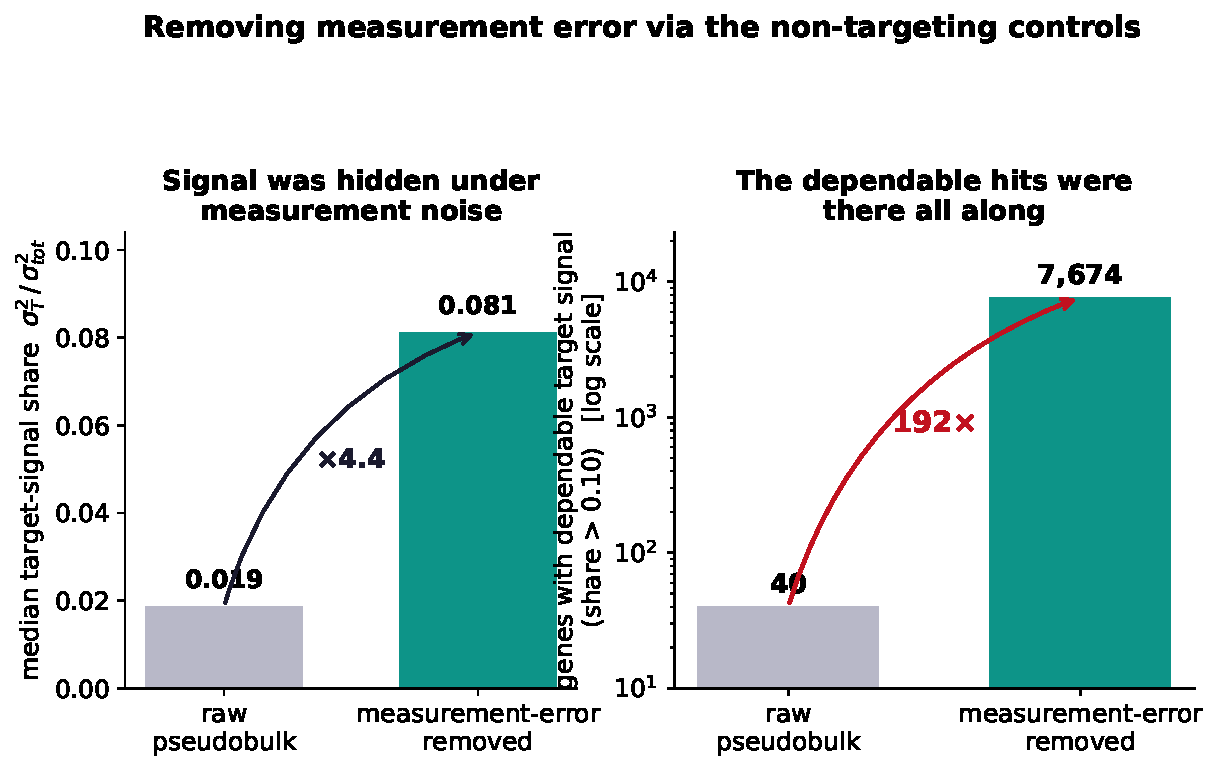
\includegraphics[width=\linewidth]{fig1_me_removal.pdf}
  \caption{Measurement-error removal via the non-targeting controls. Left, the
  median target-signal share; right, the number of genes with a dependable
  target-signal share above $.10$, on a logarithmic axis.}
  \label{fig:me}
\end{figure}

\subsection{A guide-limited design}

A design study projects the generalizability coefficient onto alternative numbers
of guides and donors (Figure~\ref{fig:dstudy}). On the representative signal genes
the current design (two guides, four donors) reaches $E\rho^2 \approx .44$. The
guide error term exceeds the donor error term by a factor of about $2.4$; adding
one guide raises the coefficient about three times as much as adding one donor.
With two guides the coefficient is capped near $.53$, and no number of donors
reaches $.70$, whereas $.70$ is attainable with about fifteen guides.
Guide-to-guide variability, rather than donor heterogeneity, is the binding
constraint, which is actionable guidance for the design of subsequent screens.
Repeating the design study within each activation state returns the same verdict
in all three states (Table~\ref{tab:percond}), so the recommendation is not an
artifact of pooling; within a state the guide term dominates the donor term more
sharply still, because most donor disagreement is a cross-state phenomenon.

\begin{figure}[t]
  \centering
  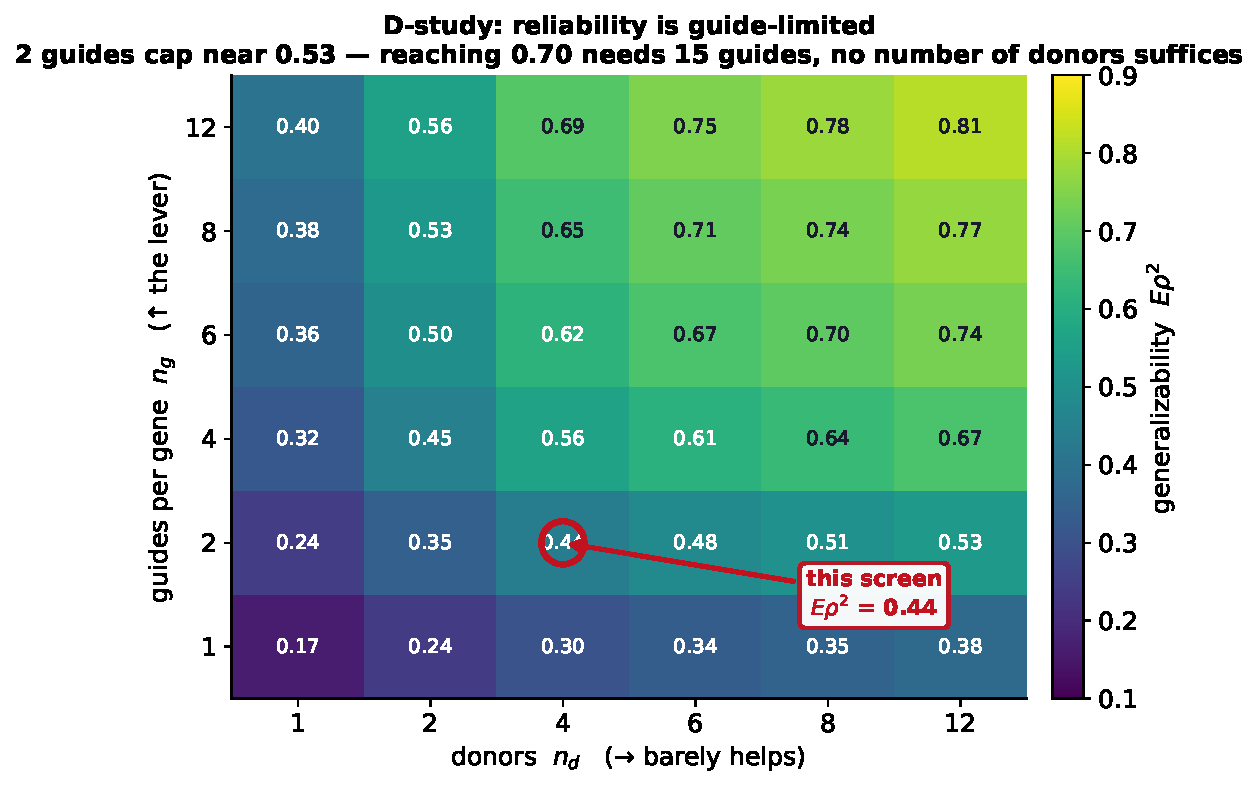
\includegraphics[width=0.82\linewidth]{fig2_dstudy_surface.pdf}
  \caption{The generalizability coefficient $E\rho^2$ across the design grid. The
  current screen (two guides, four donors) is marked; reaching $.70$ requires
  about fifteen guides and is unreachable by adding donors.}
  \label{fig:dstudy}
\end{figure}

\begin{table}[t]
  \centering
  \caption{Per-condition design study on the representative signal genes. The
  guide-limited verdict holds within every activation state.}
  \label{tab:percond}
  \begin{tabular}{lccc}
    \toprule
    Activation state & $E\rho^2$ & Guide error & Donor error \\
    \midrule
    Rest      & $.502$ & $.026$ & $.005$ \\
    Stim8hr   & $.507$ & $.023$ & $.004$ \\
    Stim48hr  & $.491$ & $.019$ & $.004$ \\
    Pooled    & $.438$ & $.040$ & $.017$ \\
    \bottomrule
  \end{tabular}
\end{table}

\subsection{A reliability-weighted ranking}

Ranking targets by $S_t$ reorders the candidate list relative to effect size
alone (Figure~\ref{fig:rank}). Of the $100$ highest-effect targets, $49$ fall out
of the $100$ most dependable, and reproducible targets that effect size underranks
rise (Table~\ref{tab:rankshift}). These are the targets a dependability-weighted
screen would nominate for validation but a strength-ranked screen would overlook.

\begin{figure}[t]
  \centering
  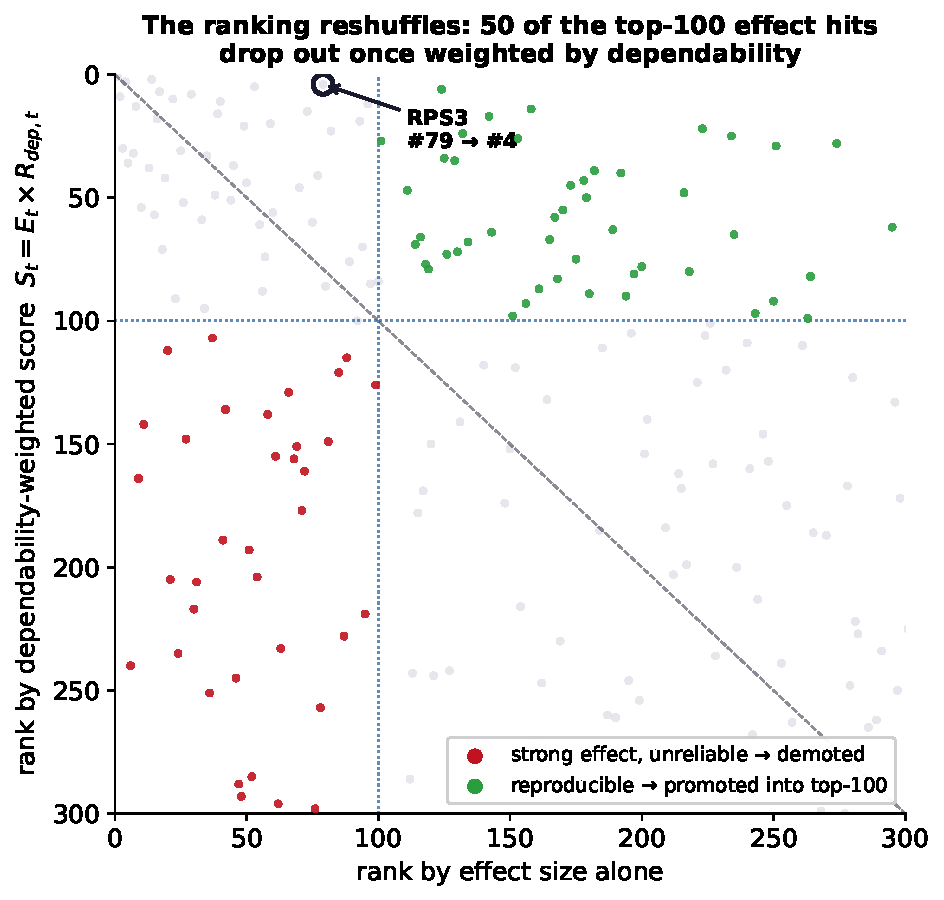
\includegraphics[width=0.78\linewidth]{fig3_ranking_reshuffle.pdf}
  \caption{Rank by effect size alone (horizontal) against rank by the
  dependability-weighted score (vertical). Points below the diagonal in the
  lower-left quadrant are demoted (strong but unreliable); points in the upper
  right are promoted (reproducible).}
  \label{fig:rank}
\end{figure}

\begin{table}[t]
  \centering
  \caption{Targets that effect size underranks but dependability promotes. Rank
  is out of the $7{,}169$ scored targets.}
  \label{tab:rankshift}
  \begin{tabular}{lccc}
    \toprule
    Target & Rank by effect & Rank by dependability & $\Rdep$ \\
    \midrule
    RPS3  & $79$  & $4$  & $.34$ \\
    QARS1 & $53$  & $5$  & $.32$ \\
    RPP21 & $124$ & $8$  & $.34$ \\
    IMP4  & $96$  & $13$ & $.31$ \\
    NMD3  & $158$ & $17$ & $.33$ \\
    \bottomrule
  \end{tabular}
\end{table}

\subsection{Context-specific dependability recovers the TCR module}

Analyzed within activation states, dependability separates targets that are
reliable across all states from targets that are reliable in one state and not
another (Figure~\ref{fig:tcr}). Because a within-state coefficient rests on
roughly a third of the cells and runs lower than the pooled value, states are
compared to one another rather than to the pooled number. One hundred targets are
context-specific in this sense. Among them, the T-cell-receptor signaling module,
the CD3 complex (CD3D, CD3G, CD247) with the proximal kinase ZAP70 and the
scaffold LAT, is reliably measurable only in activated cells, with resting
dependability at the noise floor (resting $R_{\mathrm{dep}} \approx .02$--$.05$;
stimulated $\approx .20$--$.28$). The knockdown effect for CD3D grows with
activation (effect magnitude $.26$, $.57$, and $1.12$ across Rest, Stim8hr, and
Stim48hr) and becomes dependable only upon activation. The framework reconstructs
a coherent signaling module from dependability alone, without gene annotation,
which is the strongest available evidence that it measures a real property of the
perturbation rather than an artifact of the summary.

\begin{figure}[t]
  \centering
  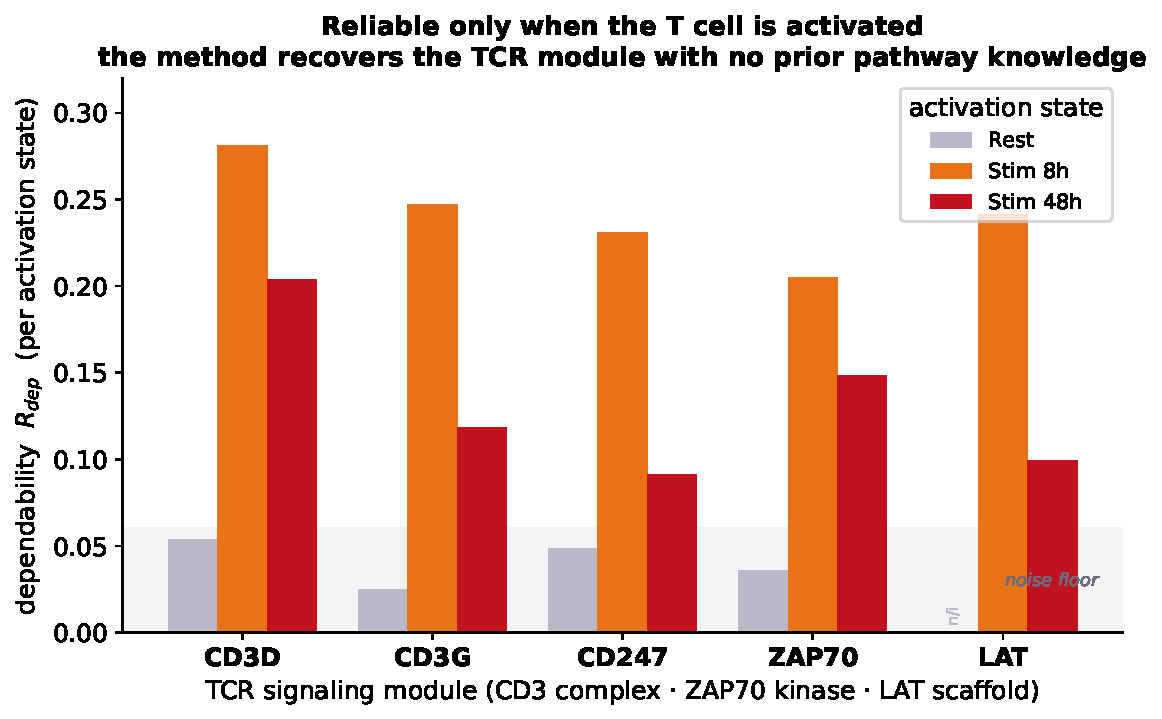
\includegraphics[width=\linewidth]{fig4_context_tcr.pdf}
  \caption{Per-state dependability for the T-cell-receptor signaling module.
  Resting values sit at the noise floor; the effect becomes reliably measurable
  only upon activation.}
  \label{fig:tcr}
\end{figure}

\section{Reproducibility}

The pipeline runs end to end from the released summary statistics, without
processing the full single-cell data: data retrieval, a checksummed evidence
manifest, identifiability gates, synthetic method selection, per-gene
decomposition, measurement-error removal, the design study, and the per-context
ranking. All results are committed as tables and figures, and every reported
number regenerates from a single re-run. The code is released under Apache-2.0.

\section{Limitations}

Four donors leave the donor variance component with three degrees of freedom, so
the donor coefficient and the donor axis of the design study carry real
uncertainty, which we report as bands rather than point values. Sequencing run is
partially confounded with donor, a fact of the released design that we record
rather than correct. A small number of full-scale Monte-Carlo gate confirmations
are scheduled on a compute cluster; the results shown are the local synthetic and
real-data tier. Finally, this is a re-analysis of released data, so the
design-study guidance is prospective, addressed to subsequent screens rather than
to the present one.

\appendix

\section{A recorded, cross-model-hardened process}

The methodology was developed under an auditable process
(Figure~\ref{fig:hardening}). Each decision --- the choice of estimator, the
thresholds, the classification of each facet as random or fixed, the criterion
for identifiability --- was recorded as a versioned issue using issue-driven
development \parencite{idd} and spec-driven development, both open-source tooling
the author maintains. Because the reasoning was documented rather than implicit,
the frozen record could be subjected to adversarial review by an independent
frontier model, which returned a blocked verdict with eleven findings, three of
them critical, spanning identifiability, measurement error, selection, validation
leakage, and compute. Each finding was resolved within the same recorded loop:
the falsification gates and controls were frozen before any real result was
inspected, the estimator was selected as in Section~3, and a mis-specified
reliability aggregation (a product of coefficients) was replaced by the joint
coefficient of Section~2.2. The resolutions were then cross-verified across models
with a second adversarial pass and with \texttt{parallel-ai-agents}
\parencite{parallelaiagents}, a package the author maintains that dispatches a task
to independent agents and cross-compares their outputs. The recorded decisions, the
blocked verdict, and every resolution are versioned in the repository.

\begin{figure}[t]
  \centering
  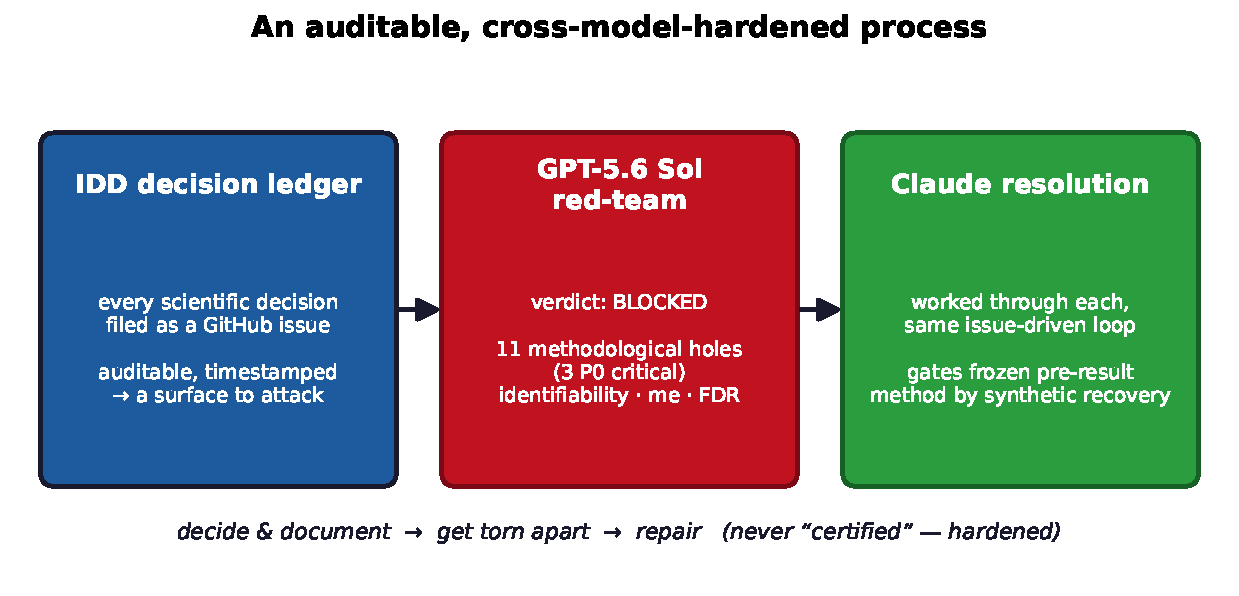
\includegraphics[width=\linewidth]{fig5_sol_hardening.pdf}
  \caption{The recorded, cross-model-hardened process: a decision ledger enables
  adversarial review by an independent model, whose blocked verdict is resolved
  in the same loop. The verdict was blocked and worked through, not certified.}
  \label{fig:hardening}
\end{figure}

\printbibliography

\end{document}
